\RequirePackage{plautopatch}
\documentclass[english, dvipdfmx, a4paper]{jsarticle}
\usepackage[utf8]{inputenc}
\usepackage[top=10truemm, bottom=20truemm, left=15truemm, right=15truemm]{geometry} % mergin
\renewcommand{\headfont}{\bfseries}
% graphics
\usepackage{graphicx}
\usepackage{here}

% link

\usepackage{tikz}
\usepackage{mathtools}
\usetikzlibrary{decorations.pathmorphing}
\usetikzlibrary{shapes}

\usepackage{url}
\usepackage[dvipdfmx, linktocpage]{hyperref} 
\usepackage{xcolor}
\usepackage{pxjahyper}
\hypersetup{
	colorlinks=true,
	citecolor=blue,
	linkcolor=teal,
	urlcolor=orange,
}

% math

\usepackage{amsmath, amssymb} 
\usepackage{physics}
\usepackage{mathrsfs}
\usepackage{mathtools}

% theoremstyle
\usepackage{amsthm}
\newtheoremstyle{break}
{\topsep}{\topsep}%
{}{}%
{\bfseries}{}%
{\newline}{}%
\theoremstyle{break}
\newtheorem{thm}{Theorem}[section]
\newtheorem{defn}[thm]{Definition}
\newtheorem{eg}[thm]{Example}
\newtheorem{cl}[thm]{Claim}
\newtheorem{cor}[thm]{Corollary}
\newtheorem{fact}[thm]{Fact}
\newtheorem{rem}[thm]{Remark}
\newtheorem{prob}{Problem}[section]

\makeatletter
\newenvironment{pr}[1][\proofnam]{\par
\topsep6\p@\@plus6\p@ \trivlist
\item[\hskip\labelsep{\itshape #1}\@addpunct{\bfseries}]\ignorespaces
}{%
\endtrivlist
}
\newcommand{\proofnam}{\underline{Derivation.}}
\makeatother


% my command
\newcommand{\e}{\mathrm{e}}
\renewcommand{\i}{\mathrm{i}}
\newcommand{\R}{\mathbb{R}}
\newcommand{\C}{\mathbb{C}}
\newcommand{\Z}{\mathbb{Z}}

\newcommand{\eq}[1]{Eq. \eqref{#1}}
\newcommand{\theorem}[1]{Thm. \ref{#1}}
\newcommand{\definition}[1]{Def. \ref{#1}}
\newcommand{\proposition}[1]{Prop. \ref{#1}}
\newcommand{\example}[1]{e.g.\ref{#1}}
\newcommand{\claim}[1]{Cl. \ref{#1}}
\newcommand{\corolary}[1]{Cor. \ref{#1}}
\newcommand{\remark}[1]{Rem. \ref{#1}}
\newcommand{\problem}[1]{Prob. \ref{#1}}
\newcommand{\slashed}[1]{#1\!\!\!/}
\renewcommand{\O}{\mathcal{O}}


% number

%\makeatletter
%\@addtoreset{equation}{section}
%\makeatother
%\numberwithin{equation}{section}
%\renewcommand{\thefootnote}{\roman{footnote}.}
%\renewcommand{\appendixname}{Appendix }

\title{How to push the contour upward?}
\author{Toshiya Tanaka}
\date{\today}

\begin{document}
	\maketitle
	\section{branch cutの見つけ方}
	複素関数で,$z^{1/2} $や$\log z $などを考えるとき,これらは多価関数になってしまうことがある.
	このような場合,定義域に複素平面を$n $枚取ってきて,適切に張り合わせたものを採用する方法をとる.
	
	この定義域をRiemann面といい,張り合わせる線をbranch cutという.
	例えば,$z^{1/2} $の場合,複素平面を二枚持ってきて,phaseが$0\to2\pi $のときを一枚目に担当させ,$2\pi $を超えると二枚目にゆき,$2\pi\to4\pi $を二枚目の複素平面が担当し,$4\pi $を超えると一枚目に戻るようにすればよい.
	このとき,branch cutは\eq{eq:1/2_branch}のように入る.
	\begin{equation}
	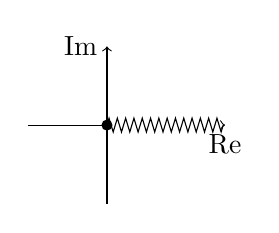
\begin{tikzpicture}
	\draw[->] (0,-1)--(0,1) node[left] {$\mathrm{Im}$};
	\draw (-1, 0) -- (0, 0);
	\fill (0, 0) circle (2pt);
	\draw[-> ,decorate, decoration={zigzag, segment length=3}](0, 0) -- (1.5, 0) node[below] {$\mathrm{Re}$};
	\end{tikzpicture}\label{eq:1/2_branch}
	\end{equation}
	また,$(z-a)^{1/2} $の場合は,$(a, \infty) $にbranch cutが入ると思えば良い.
	\section{本題}
	計算したいものは,space likeな自由場のプロパゲータ
	\begin{equation}
			D(x) = -\i\int \frac{\dd[3]{k}}{(2\pi)^32\sqrt{|\vec{k}|^2+m^2}}\e^{-\i\vec{k}\cdot\vec{x}}
	\end{equation}
	である.

	まず,球座標に変数変換して,積分する.

	\begin{align}
			D(x) &= -\i\int_{0}^{\infty}\dd{k}\int_{0}^{\pi}\dd{\theta}\int_{0}^{2\pi}\dd{\phi}k^2\sin\theta\frac{\e^{-\i\vec{k}\cdot\vec{x}\cos\theta}}{(2\pi^3)2\sqrt{k^2+m^2}}\\
				 &= \frac{1}{8\pi^2}\int_{0}^{\infty}\dd{k}\frac{k}{\sqrt{k^2+m^2}}\qty(\e^{-\i kx}-\e^{\i kx})\\
				 &= \frac{-1}{8\pi^2}\int_{-\infty}^{\infty}\dd{k}\frac{k}{x\sqrt{k^2+m^2}}\e^{\i kx}\\
				 &= \frac{\i}{8\pi^2x}\pdv{}{x}\int_{-\infty}^{\infty}\dd{k}\frac{\e^{\i kx}}{\sqrt{k^2+m^2}}.
	\end{align}

	これより,積分
	\begin{equation}
			I \coloneqq \int_{-\infty}^{\infty}\dd{k}\frac{\e^{\i kx}}{\sqrt{k^2+m^2}} 
	\end{equation}
	を計算すればよい.

	被積分関数のpoleは$k=\pm \i m $にあり,$\sqrt{k^2+m^2} = \sqrt{k+\i m}\sqrt{k- \i m} $なので,branch cutは$(-\infty, -\i m] $, $[\i m, \infty) $に取れば良い.
	
	ここで,積分路をCauchyの積分定理を用いて,次のように変形する.
	\begin{equation}
			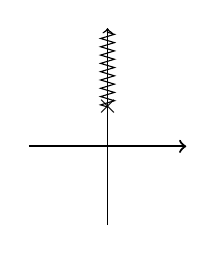
\begin{tikzpicture}
					\draw[->, thick] (-1, 0)--(1, 0);
					\draw[->] (0, -1)--(0, 1.5);
					\draw (0,0.5)node {$\times$};
					\draw[-> ,decorate, decoration={zigzag, segment length=3}](0, 0.5)--(0, 1.5);
			\end{tikzpicture}
			\quad=\quad 
			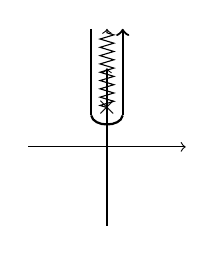
\begin{tikzpicture}
					\draw[->] (-1, 0)--(1, 0);
					\draw[->] (0, -1)--(0, 1);
					\draw[thick] (-0.2, 1.5)--(-0.2, 0.4);
					\draw[thick] (-0.2, 0.4) to [out=280, in=260](0.2, 0.4);
					\draw[thick, ->] (0.2, 0.4) -- (0.2, 1.5);
					\draw (0,0.5)node {$\times$};
					\draw[-> ,decorate, decoration={zigzag, segment length=3}](0, 0.5)--(0, 1.5);
			\end{tikzpicture}
	\end{equation}
	この操作は``push the contour upward''などと書かれる.
	注意すべきは,$k\colon \i\infty \to \i m $の経路と$k\colon \i m\to\i\infty $は同じ複素平面にあるので,定義域のphaseは$2\pi $ずれていることである.このため,被積分関数の符号が二つの経路で反転するので,
	\begin{equation}
			I = \int_{\i\infty}^{\i m}\dd{k}\frac{\e^{\i kx}}{-\sqrt{k^2+m^2}}+\int_{\i m}^{\i\infty} \dd{k}\frac{\e^{\i kx}}{\sqrt{k^2+m^2}} =2 \int_{\i m}^{\i\infty} \dd{k}\frac{\e^{\i kx}}{\sqrt{k^2+m^2}}
	\end{equation}
	となる.
	これにより,$k=\i(y+m) $と変数変換すれば
	\begin{equation}
			I = 2\int_{0}^{\infty}\dd{y}\frac{\e^{-(m+y)x}}{\sqrt{(y+m)^2-m^2}}
	\end{equation}
	となる.さらに,$y+m=u $,$u=\cosh\eta $と変数変換することで,
	\begin{align}
			I &=2 \int_{1}^{\infty} \dd{u}\frac{\e^{-mux}}{\sqrt{u^2-1}}\\
			  &=2 \int_{0}^{\infty} \dd{\eta}\e^{-mx\cosh\eta}
	\end{align}
	となる.propagatorに戻ると,
	\begin{align}
			D(x) &= \frac{\i}{4\pi^2}\pdv{}{x}\int_{0}^{\infty} \dd{\eta}\e^{-mx\cosh\eta}\\
				 &= \frac{\i}{4\pi^2}\int_{0}^{\infty}\dd{\eta}(-m\cosh\eta)\e^{-mx\cosh\eta}
	\end{align}
	となり,$\sinh\eta=s $とおくことで,
	\begin{align}
			D(x) &= \frac{-\i m}{4\pi^2}\int_{0}^{\infty}\dd{s}\e^{-mx\sqrt{1+s^2}}\\
				 &\simeq \frac{-\i m}{4\pi^2}\frac{1}{2}\sqrt{\frac{2\pi}{mx}}\e^{-mx}\\
				 &= \frac{-\i m^2}{4\pi^2}\sqrt{\frac{\pi}{2(mx)^3}}\e^{-mx}
	\end{align}
	となり,空間方向には$\e^{-mx} $程度しか伝播しないことがわかる.
	%\bibliography{}
	%\bibliographystyle{ytamsalpha}
	%\bibliographystyle{ytamsbeta}
\end{document}

